\documentclass[]{standalone}
\usepackage[utf8]{inputenc}
\usepackage[american]{circuitikz}
\usetikzlibrary{arrows,shapes,calc,positioning}

\begin{document}

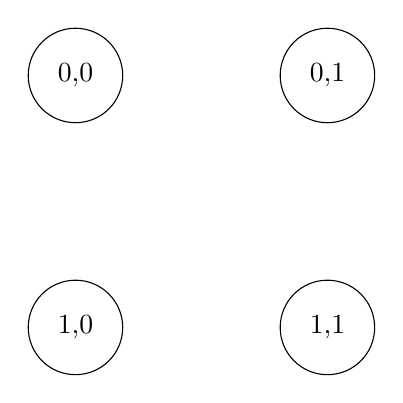
\begin{tikzpicture}[scale=1, node distance=32mm]
  \node[circle, draw, minimum height=12mm] (ab00) {0,0};
  \node[circle, draw, minimum height=12mm, right of=ab00] (ab01) {0,1};
  \node[circle, draw, minimum height=12mm, below of=ab01] (ab11) {1,1};
  \node[circle, draw, minimum height=12mm, left of=ab11] (ab01) {1,0};
\end{tikzpicture}
\end{document}
